\documentclass{article}
\usepackage[utf8]{inputenc}
\usepackage{graphicx}
\usepackage{titlepic}
\usepackage{hyperref}
\usepackage{xcolor}
\usepackage{amsmath}
\usepackage{textcomp}

\titlepic{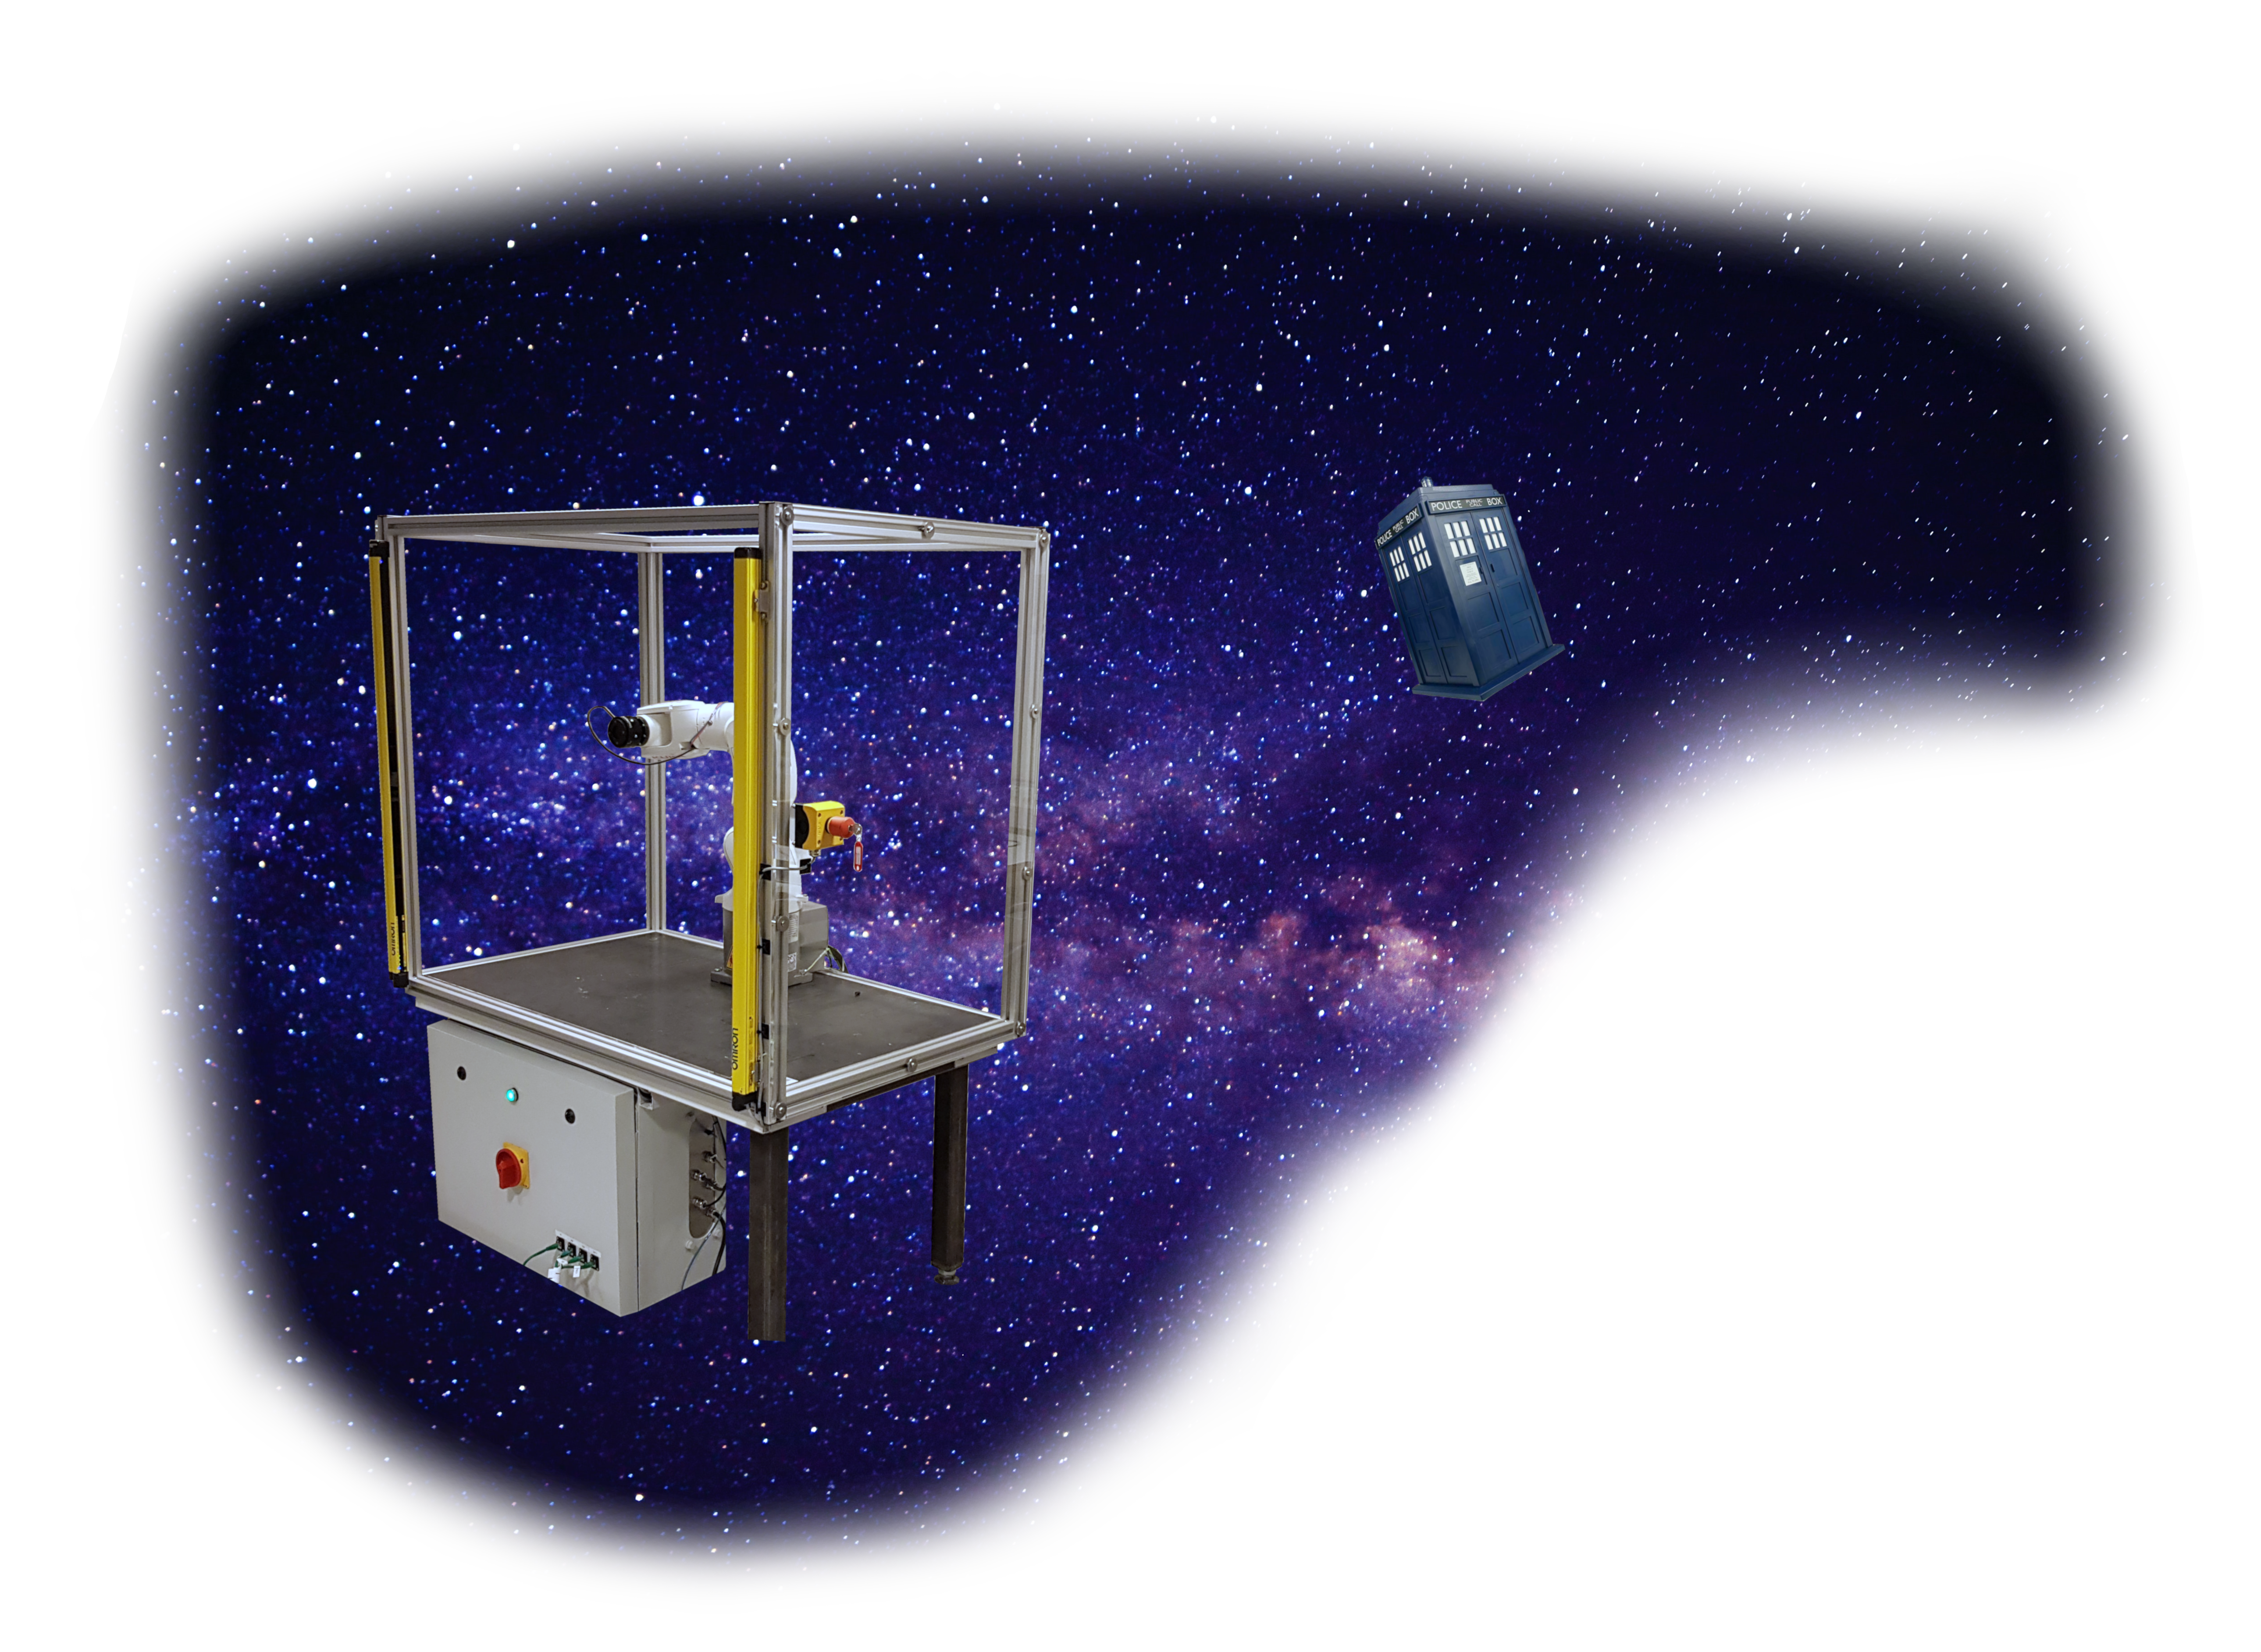
\includegraphics[width=\textwidth]{Pictures/robotlab1_final.png}}
\title{Getting started with Kuka Robot Cell}
\author{Espen Teigen }
\date{March 2019}


\begin{document}

\maketitle

    Github: https://github.com/EspenTeigen/Kuka-KR-C4-commissioning

\newpage
\tableofcontents{}
\newpage


\section{Overview of the Robot-cell and it's parts}
    \subsection{Manipulator}
    
     \begin{figure}[!h]
        \centering
        \includegraphics[scale=0.09]{"Pictures/KR_3_AGILUS".jpg}
        \caption{Kuka KR 3 R540 Agilus}
    \end{figure}
    
    
    Ahh... The manipulator, the part that everyone thinks is the robot, but no. A robot consists of a controller, effector and a manipulator, but I am getting ahead of myself.
    \\\\
    The manipulator is the part that delivers the movement of the tool. In it self, it is just a collection of motors and joints, or as the robotics companies like to say "jointed-arm kinematic system". 
    \newpage
    This manipulator is:
    \begin{itemize}
        \item 6-axis
        \item Capable of moving 3kg of mass(included tool)
        \item Giving a $\pm 0.02mm$ pose repeatabillity
        \item Weighing 26.5kg without a tool
        \item Not very big. It has a maximum reach of 541mm(without tool)
        \item Silent, less then 68dB
        \item Made for pairing with the KR C4 compact controller
        \item What we would call an assembly robot
        \item Really, really fast(See KR 3 R540 Operating Instructions page 12)
        \item In my opinion, really good looking
    \end{itemize}
    
    \\\\
    It is not:
    \begin{itemize}
        \item A pot of petunias falling to the ground
        \item A time traveling  TARDIS\textsuperscript{TM}
        \item A toy. When the manipulator is moving at full speed, it has the power to do some major damage to both humans and equipment. Never try to override the safety system, and keep body parts away from the robot cell. Try to avoid standing in front of the robot cell when the robot system are in operation, if you are not sure about how the robot is moving. 
    \end{itemize}
   
    
        \subsubsection{Force-torque sensor}
        \subsubsection{Pneumatic's}

    \subsection{Robot Controller}
        \subsubsection{SmartPad}
        \subsubsection{PC-interface}
        \paragraph{Software}
        \subsubsection{EtherCAT}
        


    \subsection{Control cabinet}
        \subsubsection{Front panel}
        \subsubsection{PLC}
        \paragraph{PC-interface}
        \paragraph{Software}
        \subsubsection{Pneumatic's}
    
    \subsection{Safety}
        \subsubsection{Do's and dont's }
        \subsubsection{Emergency stop's}
        \subsubsection{Light grid}


\end{document}
